\documentclass[letterpaper,twocolumn,10pt]{article}

% Load 'xcolor' with the 'table' option here, before any other packages.
\usepackage[table]{xcolor}

% Now load 'usenix-2020-09' and other packages.
\usepackage{usenix-2020-09}
\usepackage{tikz}
\usepackage{amsmath}
\usepackage{multirow,booktabs}
\usepackage{xspace}
\usepackage[utf8]{inputenc}
\usepackage{longtable}
\usepackage{lipsum}  % This package provides filler text.

% The 'float' and 'array' packages should not conflict with 'xcolor'.
\usepackage{float}
\usepackage{array}

% Additional packages.
\usepackage[margin=1in]{geometry} % Adjust the page margins if needed
\usepackage{tabularx} % For tables that span the width of the page
\usepackage{ltablex} % Allows 'tabularx' environments to break over pages
\usepackage{booktabs} % For better-looking tables
\usepackage{makecell} % Allows line breaks within table cells

\newcommand{\ricky}[1]{\textit{\textcolor{teal}{#1}}}
\newcommand{\echont}{\emph{NT-A}\xspace}
\newcommand{\johnnt}{\emph{NT-B}\xspace}
\newcommand{\ucsdnt}{\emph{NT-C}\xspace}
\providecommand{\eg}{\emph{e.g.,} }
\providecommand{\etc}{\emph{etc.}}      % No trailing space here either

%-------------------------------------------------------------------------------
\begin{document}
%-------------------------------------------------------------------------------

%don't want date printed
\date{}

% make title bold and 14 pt font (Latex default is non-bold, 16 pt)
\title{\Large \bf Telemetry from DDOS Protection Sevices Providers}

%for single author (just remove % characters)
\author{} % end author

\maketitle


\section{DDOS protection Services Provider (DPS)}\label{sec:DPS}
DDoS Protection Service (DPS) providers mitigating DDoS attacks through scrubbing centres, DPS can be categorized into BGP-based and DNS-based services BGP-based DPS \cite{tung2018understanding}. is favoured for large-scale attacks, leveraging the Border Gateway Protocol to reroute overwhelming malicious traffic from the victim's network to more resilient networks, significantly reducing the attack's impact.

Conversely, DNS-based DPS utilizes DNS redirection, altering the DNS records of the target domain to reroute traffic to the DPS provider’s servers. This method filters traffic, removing malicious activities and ensuring only legitimate traffic reaches the target. It hinges on changing DNS resolution, directing domain requests to DPS servers instead of the target's original servers.

\section{BGP-Based DPS: Benefits and Limitations}\label{sec:BDPS_benefits}
BGP-based DPS excels in mitigating large-scale volumetric attacks. Utilizing the Border Gateway Protocol, it diverts malicious traffic from the victim's network to robust networks equipped for traffic scrubbing. This strategy effectively diminishes the attack's impact and upholds the integrity of the target network, making it a preferred solution for defending against significant DDoS threats. However, implementing BGP-based DPS requires a substantial network infrastructure, typically involving extensive connectivity through multiple transits, Private Network Interconnects (PNI) \cite{chatzis2013there}., and Network Access Points (NAPs), leading to significant investment requirements. Moreover, there is a minimum network size constraint: the network must possess at least a Class C /24 prefix for public internet propagation, as this is the smallest network prefix that can be propagated on the public internet via BGP routing \cite{caesar2005bgp}. Smaller networks, which do not have a /24 network or larger, might find this requirement challenging, limiting the feasibility of BGP-based DPS for such organizations.

\section{DNS-based DPS: Benefits and Limitations}\label{sec:DDPS_benefits}
DNS-based DDoS Protection Services (DPS) offer effective mitigation strategies by modifying the address record (A-record) in the target's DNS server \cite{schomp2020akamai}. The strategic adjustment of the Time-To-Live (TTL) values facilitates rapid updates and propagation of DNS records, which is essential in rerouting traffic efficiently during an attack. This method proves especially beneficial for web portals or applications dependent on DNS for reachability, offering a viable solution for small and medium-sized enterprises (SMEs) or organizations with smaller network infrastructures, as it does not necessitate a /24 network prefix. However, the effectiveness of DNS-based DPS is constrained when facing direct-to-IP attacks. Such attacks include services like FTP (File Transfer Protocol), SSH, SMTP (Simple Mail Transfer Protocol) for email, or other proprietary protocols often used in enterprise applications. Given that these services typically operate using fixed IP addresses rather than DNS lookups, DNS-based DPS may struggle to adequately mitigate attacks targeting them.


\section{Operational Strategies: Detection and Mitigation}\label{sec:operations}
BGP-Based DPS operational strategies are designed to address high-volume attacks targeting network bandwidth. These services utilize a comprehensive detection approach that encompasses Deep Packet Inspection (DPI), netflow analysis, and traffic graph examination \cite{wang2018delving} \cite{saied2016detection}. DPI, including critical payload inspection, is essential in accurately identifying Layer 3 and 4 attacks and is central to attack traffic fingerprinting, providing in-depth information crucial for the mitigation process. DPI's ability to delve into the specifics of packet content makes it an invaluable tool in distinguishing between attack and legitimate traffic. Complementing DPI, netflow and traffic graphs offer insights into traffic flow characteristics and aid in profiling normal legitimate user traffic. This helps in detecting anomalous patterns indicative of DDoS activities. Nonetheless, DPI strategies come with limitations, including their complexity, computational demands, and challenges in analyzing encrypted traffic.

Table \ref{tab:ddos_attack_vectors} provides a list of 73 attack vectors identified by a DPS from 1 Jan 2019 – 31 Dec 2023


\begin{table}[!htbp]
\caption{DDoS Attack Vectors}
\label{tab:ddos_attack_vectors}
\centering
\begin{tabular}{|>{\raggedright\arraybackslash}p{2.7cm}|>{\raggedright\arraybackslash}p{4.8cm}|}
\hline
\textbf{Category} & \textbf{Attack Vectors} \\
\hline
Reflection Attack & Memcached Reflection, DNS Reflection, NTP Reflection, SSDP Reflection, CLDAP Reflection, WSDiscovery Reflection, Censorship TCP Reflection, TFTP Reflection, mDNS Reflection, Netbios Reflection, ARMS Reflection, SNMP Reflection, RPC Reflection, SQL Server Reflection, RIP Reflection, SADP Reflection, SLP Reflection, Ubnt Reflection \\
\hline
Network Layer Attack & GRE Protocol Flood, ICMP Flood, IGMP Flood, IP Fragment \\
\hline
Transport Layer Attack (UDP) & UDP Flood, UDP Fragment \\
\hline
Transport Layer Attack (TCP) & TCP Anomaly, ACK Flood, SYN Flood, PSH ACK Flood, RESET Flood, SYN ACK Flood, Reserved Protocol Flood, TCP Fragment, Connection Flood, PUSH Flood, FIN Flood, XMAS, FIN PUSH Flood \\
\hline
Application Attack (UDP) & DNS Flood, NTP FLOOD, CharGEN Attack, SSDP Flood, DHdiscovery, STUN, SNMP Flood, Netbios Flood, mDNS Flood, TFTP Flood, ESP Flood, HEAD Flood, RIP Flood, coap, quake, voip10074 \\
\hline
Application Attack (TCP) & HTTP Flood, Apple Remote Desktop, Sentinel Flood, valvesrcds, VxWorks, afs, steamremoteplay, nat pmp, ikev1, plex, TLS Exhaustion, fivem, GET Flood, SSL GET Flood, POST Flood, SSL POST Flood \\
\hline
Others & SYN PUSH, WSDiscovery Flood \\
\hline
\end{tabular}
\end{table}



In contrast, DNS-Based DPS targets application-layer attacks and emphasizes analyzing content requests \cite{xie2008monitoring}. Unlike Layer 3 or 4 attacks where DPI provides significant benefits, application-layer attack detection in DNS-based DPS can rely on sufficient telemetry from traffic graphs and netflow analysis without necessitating DPI. This is particularly relevant when the network traffic is unrelated to the application layer, such as UDP packet floods or TCP packets on unrelated ports, which are not pertinent for a targeted web server's DPI analysis. DNS-based DPS instead places a greater emphasis on application logs from targeted systems. These logs are pivotal in identifying activities that exploit application vulnerabilities or functionalities, offering direct insights into how the application is being manipulated or overwhelmed by attack traffic. While DPI offers thorough traffic analysis, its effectiveness for DNS-based DPS is limited due to the complexities and demands of DPI, and its limited utility in encrypted traffic analysis.

Table \ref{tab:application_attacks} provided a list of application based attack vectors (strategy) \cite{zolotukhin2018data} which are the primary focus of DNS-Based DPS.

\begin{table}[!htbp]
\centering
\caption{Summary of Application Layer Attack Vectors}
\begin{tabular}{|p{0.3\linewidth}|p{0.6\linewidth}|}
\hline
\textbf{Category} & \textbf{Attack Vectors} \\
\hline
Application Layer Attack (HTTP/HTTPS) & Slowloris, HTTP Flood, HTTPS Flood, HTTP/2 Flood, POST Flood, GET Flood, SSL Renegotiation Attack, SSL Exhaustion, HTTP Parameter Pollution, HTTP Bomb \\
\hline
Application Layer Attack (Web Applications) & Cross-Site Scripting (XSS), SQL Injection, Cross-Site Request Forgery (CSRF), Remote File Inclusion (RFI), Local File Inclusion (LFI), XML External Entity (XXE) Attack \\
\hline
Application Layer Attack (API) & API Endpoint Abuse, Excessive API Rate, GraphQL Injection, REST API Manipulation \\
\hline
Application Layer Attack (Authentication) & Credential Stuffing, Brute Force Attack, Dictionary Attack, Password Spraying \\
\hline
Application Layer Attack (CMS) & WordPress XML-RPC Flood, Joomla! SQL Injection, Drupalgeddon, Magento SQL Injection \\
\hline
Application Layer Attack (Frameworks) & Struts RCE Exploit, Ruby on Rails Code Injection, Node.js Route Enumeration \\
\hline
Application Layer Attack (Email Services) & Mail Bombing, Spamming, Phishing Attack, Email Spoofing \\
\hline
Application Layer Attack (DDoS Bots) & Mirai Botnet, Bashlite Botnet, Tor's Hammer, HOIC, LOIC \\
\hline
Miscellaneous Application Attacks & WebSocket Flood, Malicious Bot Scraping, Drive-By Download, Clickjacking \\
\hline
\end{tabular}
\label{tab:application_attacks}
\end{table}


\section{The telemetry discrepancy among DPS in the industry}\label{sec:telemetry}
The telemetry discrepancy between BGP-Based and DNS-Based DDoS Protection Services (DPS) is primarily attributed to the difference in detection and mitigation strategies across various OSI layers and the distinct nature of their customer bases. 
\paragraph{Scope and Target Audience Differences} BGP-Based DPS, focusing on network prefixes, caters predominantly to large corporations and enterprises. Within a single network prefix, BGP-Based DPS addresses a multitude of entities spanning different network, transport, and application protocols. Conversely, DNS-Based DPS typically provides services per application, often associated with a single IP address, as outlined in the operational strategies section. 

\paragraph{Balancing Volumetric Protection and Application Layer Control} Additionally, customers utilizing BGP-Based DPS, such as financial institutions, government bodies, and banks, may seek volumetric protection while retaining control over their application layer. For instance, banking customers might be reluctant to share SSL certificates for their portals with the DPS, preferring to maintain exclusive control over the decryption of application content and requests.
\section{Industry Trends: Offering Hybrid DPS Solutions}\label{sec:solutions}
Some DPS providers in the industry are now offering both BGP-based and DNS-based services to provide a comprehensive DDoS mitigation portfolio. This hybrid approach allows for a more versatile defense strategy, catering to a broader range of attack vectors and offering tailored solutions based on the specific needs and infrastructure of the client.

Table \ref{tab:ddos_protection_services} provides a summary the commonly available DDOS solutions in the industry

\begin{table*}[t] % Use 't' to position at the top of the page
\small % Adjust the font size as necessary
\caption{Comparison of DDoS Protection Services}
\label{tab:ddos_protection_services}
\begin{tabularx}{\textwidth}{|X|X|X|X|X|}
\hline
\thead{Service Type} & \thead{General Description} & \thead{Services Protected\\ (Focus)} & \thead{Limitations} & \thead{Benefits} \\
\hline
BGP-based DPS & Offers DDoS protection for network service providers, hosting, and cloud service providers. Specifically designed to protect against a wide range of DDoS attacks by filtering malicious traffic in the cloud. & Network infrastructure, hosting services, and cloud platforms. & Reliant on BGP routing, which can be complex; limited to /24 prefixes or larger. & Effective for large-scale protection; can handle massive volumes of traffic; reduces the risk of network overload. \\
\hline
On-premises Solutions & Provides DDoS protection through physical or virtual systems installed on the client's premises. These systems can be from any vendor and are designed to integrate with the client's existing network infrastructure. & Internal networks, specific applications, and servers within the client's control. & Can be resource-intensive; may not handle large-scale attacks well; requires ongoing maintenance. & Direct control over the protection measures; immediate response to attacks; customizable to specific network needs. \\
\hline
DNS-based DPS & Protects your digital estate with a product combining a web application firewall, bot mitigation, API security, and Layer 7 DDoS protection. Utilizes DNS redirection to divert attack traffic for cleansing and protection. & Web applications, APIs, and digital platforms. & Dependent on DNS functionality; might not cover non-web-based services. & Comprehensive protection for web assets; scalable; effective against sophisticated attacks. \\
\hline
Hybrid Solution & Integrates cloud-based, on-premises DDoS protection, and/or DNS-based DPS. Leverages the strengths of various solutions for a comprehensive approach. & Combination of network infrastructure, internal networks, web applications, and cloud services. & Complexity in integrating different solutions; can be costlier. & Versatile and comprehensive protection; scalable; balances immediate on-site response with large-scale cloud capabilities. \\
\hline
\end{tabularx}
\end{table*}
\section{Mapping victims with Telescopes and Honeypot}\label{sec:mapping_victim}
This analysis establish a relationship between our recorded DDOS event data and the Telescopes and  Honeypots datasets. It specifically focuses on aligning full-day dates, spanning from midnight to the end of the day, with our defined intervals of DDOS events, as marked by startTime and endTime. 
In Telescopes' operational design, attacks are detected by analyzing backscattered traffic. This traffic typically results from attack traffic that spoofs its source address to resemble that of the Telescopes' address blocks. Based on this detection method, we can anticipate two primary scenarios:
Due to our mitigation mechanisms, there is only a slim chance that the date recorded by Telescopes will coincide with our event dataset. If Telescopes record a date that precedes the startTime and endTime of a DDOS event, it might be indicative of an attack being detected early by the Telescopes. Following this early detection, mitigation measures might be activated within the DDOS event window to address the attack. On the other hand, if a date recorded by Telescopes falls after the DDOS event timeframe, it could imply a re-emergence of the attack, occurring after the mitigation measures detailed in the DDOS event data.
The Honeypots dataset, however, provides a contrasting perspective. Unlike Telescopes, Honeypots are not just detection tools; they actively participate in attack mechanisms. As such, their data might align with DDOS events by coincidence. The occurrence of a Honeypot record during a DDOS event does not inherently suggest a direct link with the event's mitigation processes, as Honeypots operate independently of these countermeasures
\begin{figure}[htbp]
    \centering
    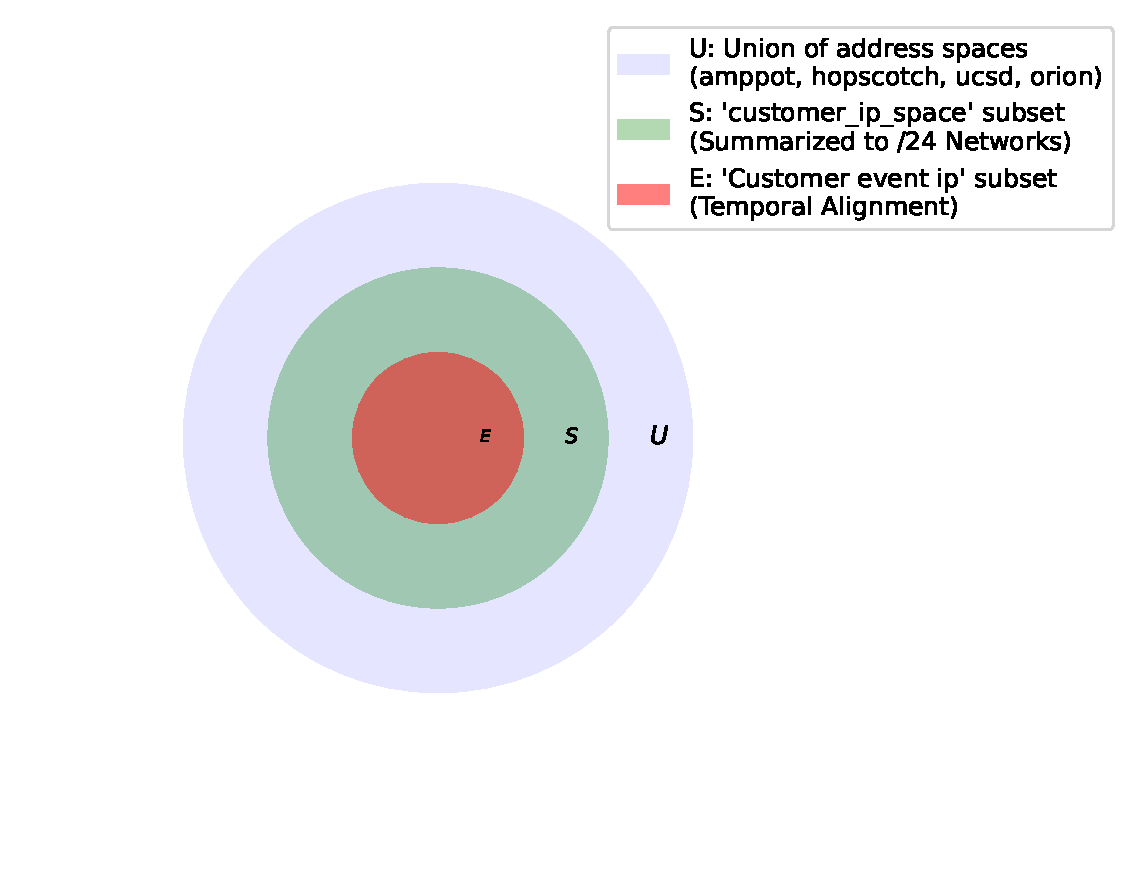
\includegraphics[scale=0.5]{graphs/sets.pdf}
    \caption{Address sets relationship}
    \label{fig:addresssets}
\end{figure}

\subsection*{'Customer IP Space $S$' Definition}
\begin{figure}[htbp]
    \centering
    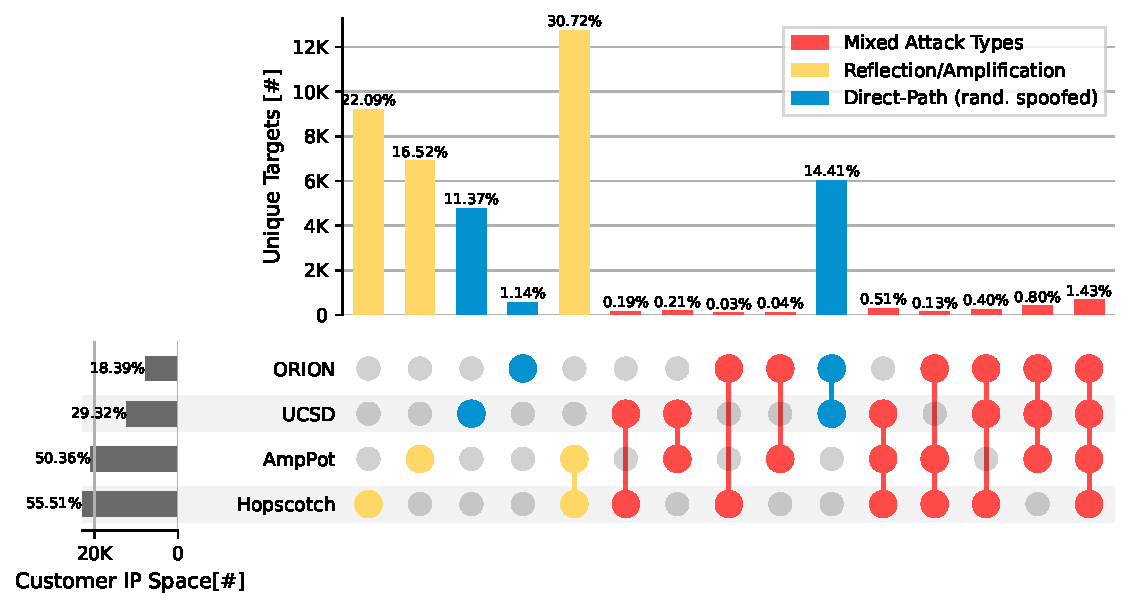
\includegraphics[scale=0.4]{graphs/space_no_event.pdf}
    \caption{Customer IP Space Analysis.}
    \label{fig:customeripspace}
\end{figure}
Fig. \ref{fig:customeripspace} shows the attack event detected by telescopes and honeypots for our interested ip space $S$.
    
Let $U$ represent the union of address spaces from the categories 'amppot', 'hopscotch', 'ucsd', and 'orion'. The 'customer\_ip\_space' condition identifies a subset of $U$, denoted as $S$, characterized by the following criteria:
\begin{enumerate}
    \item \textbf{Summarization to Class C Networks}: Each IP address in $S$ is summarized to a Class C network, represented by the first three octets of the IP address, effectively transforming the address into a /24 network notation.
    \item \textbf{Match with Summarized /24 Networks}: An address $s \in S$ is considered part of 'customer\_ip\_space' if its summarized /24 network matches with any summarized /24 network within $U$.
\end{enumerate}

\subsection*{'Customer event ip $E$' Definition}
\begin{figure}[htbp]
    \centering
    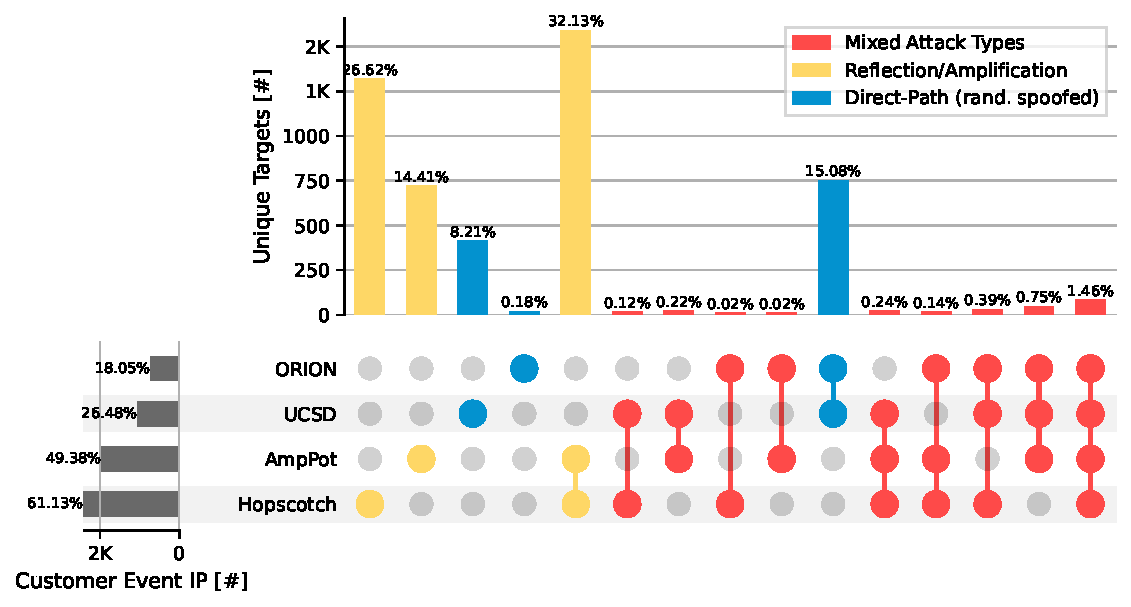
\includegraphics[scale=0.4]{graphs/space_event.pdf}
    \caption{Customer Event IP Analysis.}
    \label{fig:customereventip}
\end{figure}
Fig. \ref{fig:customereventip} shows the attack event detected by telescopes and honeypots for our interested ip attack events $S$.


Fig. \ref{fig:Mappedaddressanalysis} shows summarised the analysis of Customer IP Space, $S$ and Customer Event IP $E$.


The 'Customer event ip' condition extends the identification of relevant IP addresses by incorporating temporal alignment with specific events. It represents a subset of 'customer\_ip\_space', denoted as $E$, with the following additional condition:

\begin{enumerate}
    \item \textbf{Temporal Alignment with Events}: For an address $e \in E$, not only must it satisfy the 'customer\_ip\_space' criteria, but it must also coincide with an event whose duration ($p$) matches a specified date ($d$). The event duration is defined by the start and end times of activity associated with the IP address. An event is considered to match if $d$ falls within this duration, indicating that the event occurred within the specified timeframe.
\end{enumerate}
Fig. \ref{fig:addresssets} shows relationship among the $U$ $S$ $E$.

\begin{figure}[htbp]
    \centering
    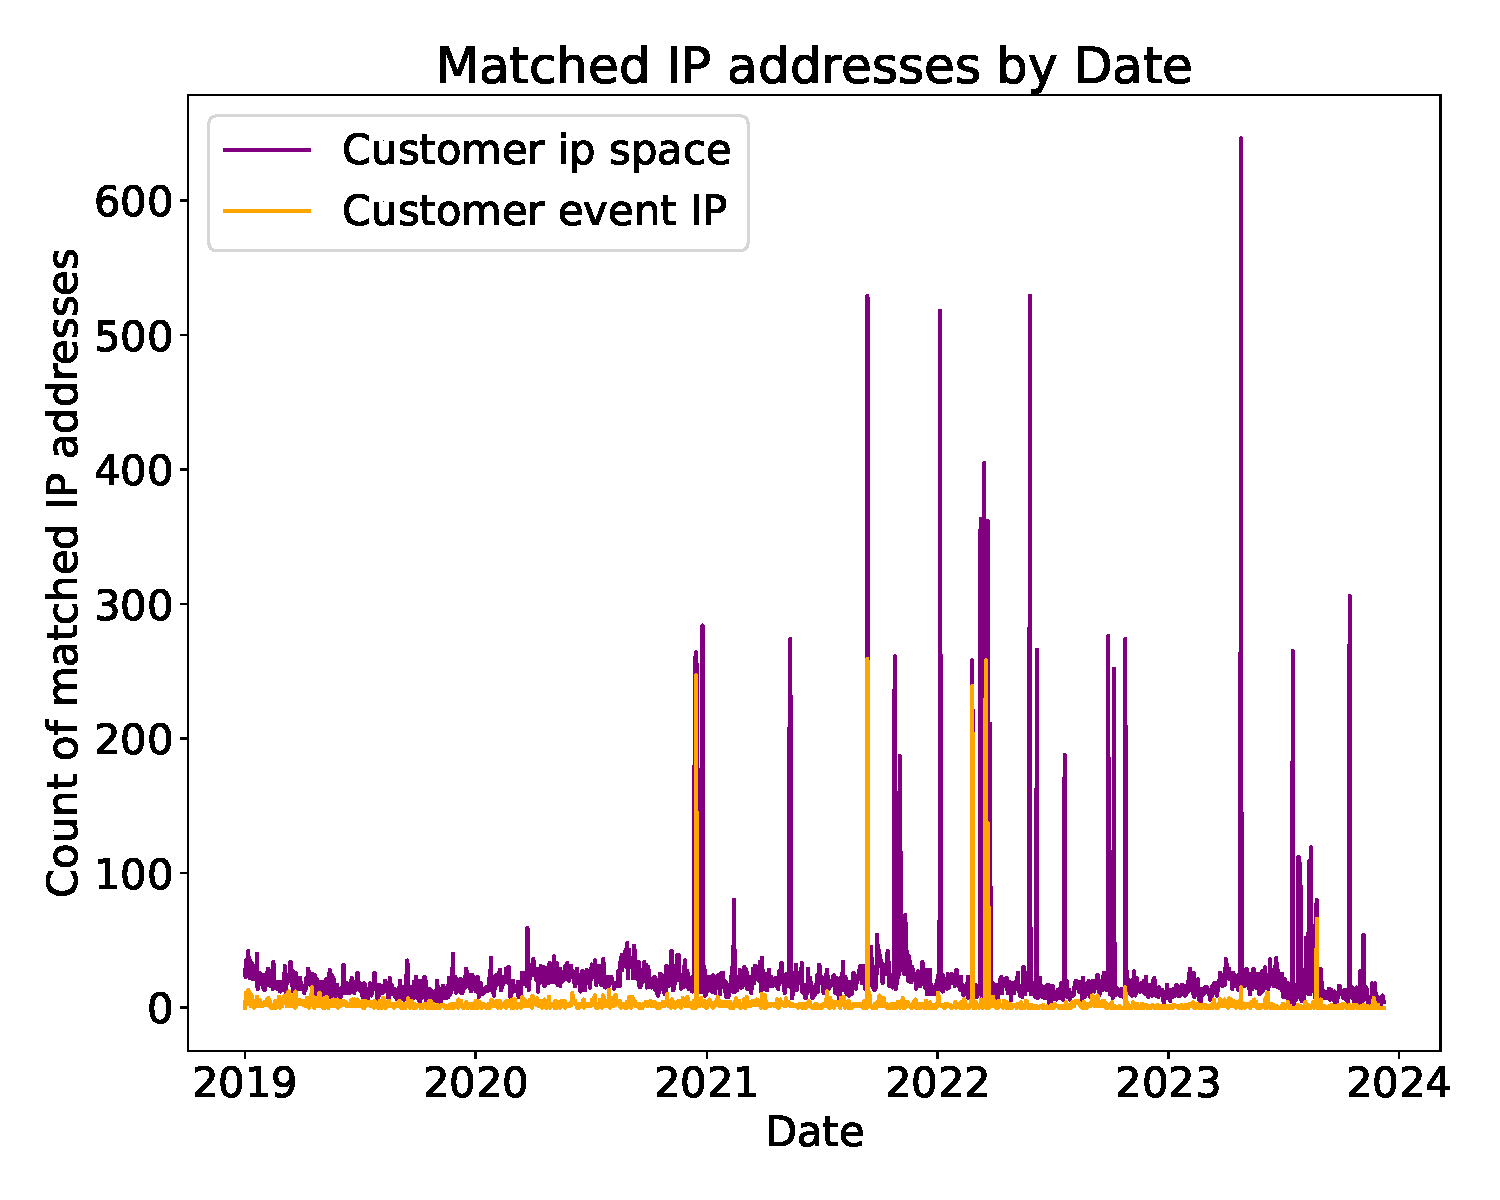
\includegraphics[scale=0.30]{graphs/matched_customer_graph.pdf}
    \caption{Mapping customer ip space and event.}
    \label{fig:mappedcustomergraph}
\end{figure}

\begin{figure*}[htbp]
    \centering
    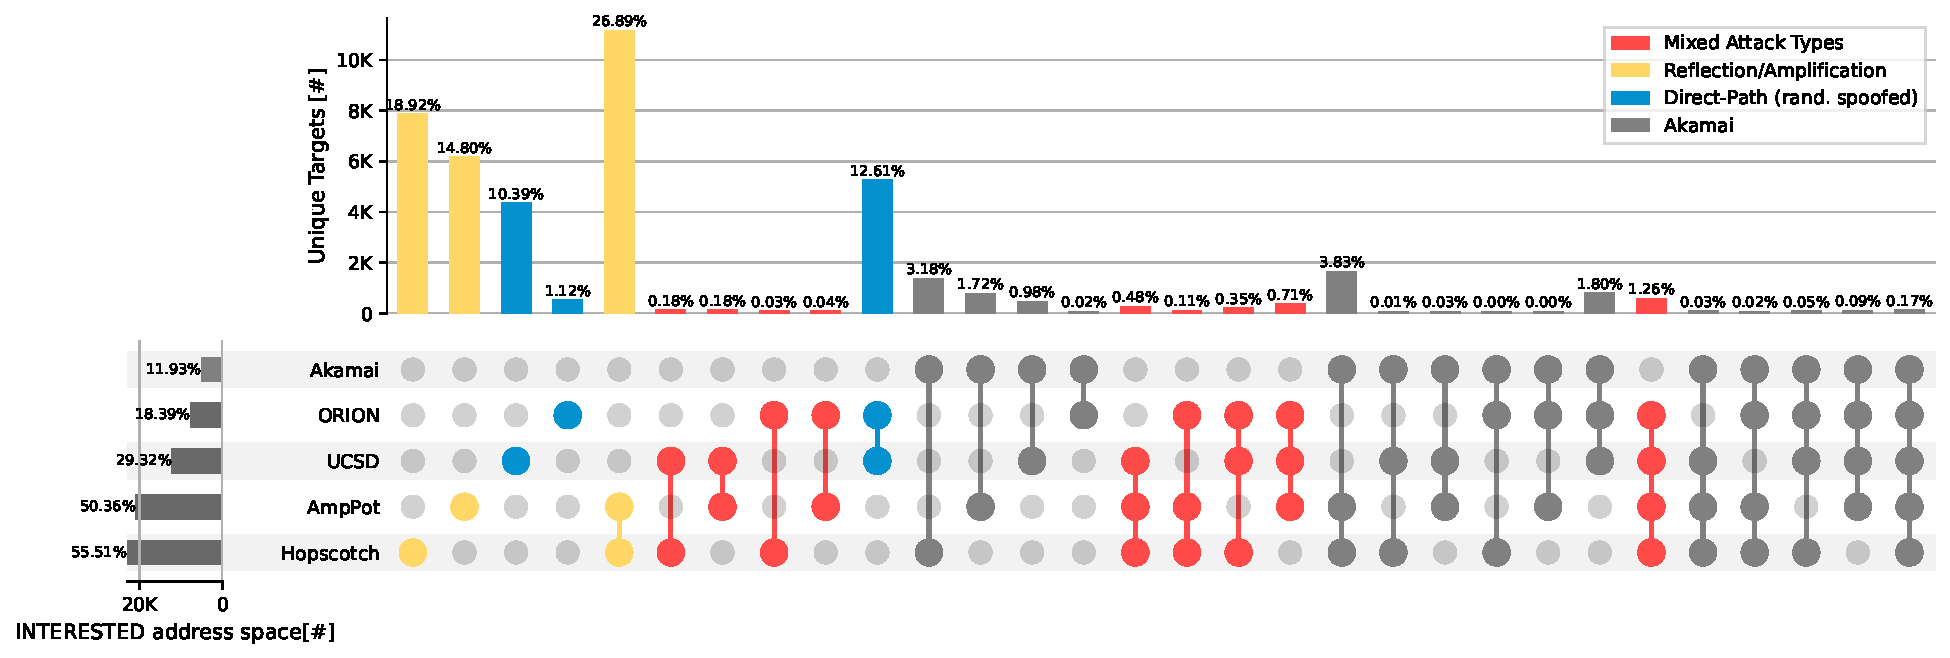
\includegraphics[scale=0.48]{graphs/noir3.pdf}
    \caption{Customer IP Space and event Analysis.}
    \label{fig:Mappedaddressanalysis}
\end{figure*}

\section{Attack Incidents Analysis}\label{sec:attackeventsfromcustomeripspace}
Fig. \ref{fig:mappedcustomergraph} visualizes the count of matched IP addresses over time, distinguishing between "Customer IP Space" and "Customer Event IP". It shows spikes indicating significant events: (A) a large number of targets detected from the Customer IP Space $S$ by telescopes/honeypots and (B) a large number of targets from Customer Events records by the DPS coincided with the telescopes/honeypots, address space $E$.

\subsection{Spikes Detected by Amppot, Hopscotch, UCSD, and Orion}
Table \ref{table:spikes_data} presents the recorded spike events, indicating that some attack events can be detected by telescope setups, while others are detected by honeypot setups.
\begin{itemize}
    \item \textbf{Telescope Detection:} UCSD and Orion identify spoofed attacks targeting IP subnets, manifested as backscattered traffic. This phenomenon is observed in two specific scenarios:
    \begin{enumerate}
        \item When a customer transitions to DDoS Protection Services (DPS) for mitigation.
        \item Before the DPS mitigation measures take effect.
    \end{enumerate}
    
    \item \textbf{Honeypot Detection:} Amppot and Hopscotch detect direct and reflection attacks, actively engaging with all IP addresses within the targeted subnets. 
\end{itemize}


\begin{table*}[htbp]
    \centering
    \caption{Matched IP counts showed as spikes in Fig \ref{fig:mappedcustomergraph}}
    \begin{tabular}{|l|l|r|r|r|r|r|}
    \hline
    \textbf{Date} & \textbf{Victim Subnet} & \textbf{Amppot} & \textbf{Hopscotch} & \textbf{UCSD} & \textbf{Orion} & \textbf{Akamai} \\
    \hline
    2020-12-15 & Subnet A & 83 & 246 & 0 & 0 & 246 \\
    2021-09-12 & Subnet B & 0 & 0 & 256 & 256 & 256 \\
    2022-02-25 & Subnet C & 1 & 1 & 239 & 0 & 239 \\
    2022-03-18 & Subnet D & 1 & 256 & 1 & 1 & 256 \\
    2022-03-22 & Subnet D & 0 & 135 & 1 & 1 & 135 \\
    2023-08-24 & Subnet E & 0 & 0 & 66 & 66 & 66 \\
    \hline
    \end{tabular}
    \label{table:spikes_data}
    \end{table*}


Please be noted that The data from the telescopes/Honeypots, which aligns with our DDOS events, is vividly represented by the spikes Customer IP Space in this context identifies IP addresses of our customers that are detected and logged within the telescopes/honeypot datasets. 
The designation Customer Event IP, however, is more specifically applied to those customer IPs that not only appear in the telescopes/honeypot datasets but also coincide with the broader timeframes delineated by the \texttt{startTime} and \texttt{endTime} of our DDOS events. Crucially, this correlation is not based on exact hour, minute, and second details, since the telescopes/honeypot data does not include these precise time elements. Rather, matching is determined by the day, with the assumption that each recorded date encompasses the full 24-hour span from one midnight to the next.

Fig \ref{fig:akamai_spikes} shows the distribution of attacks grouped by date and subnet detected by the telescopes/honeypots in the Customer IP Space sorted by the number of targeted Customer Event IP in ascending order (bin sizes).
\begin{figure*}[htbp]
    \centering
    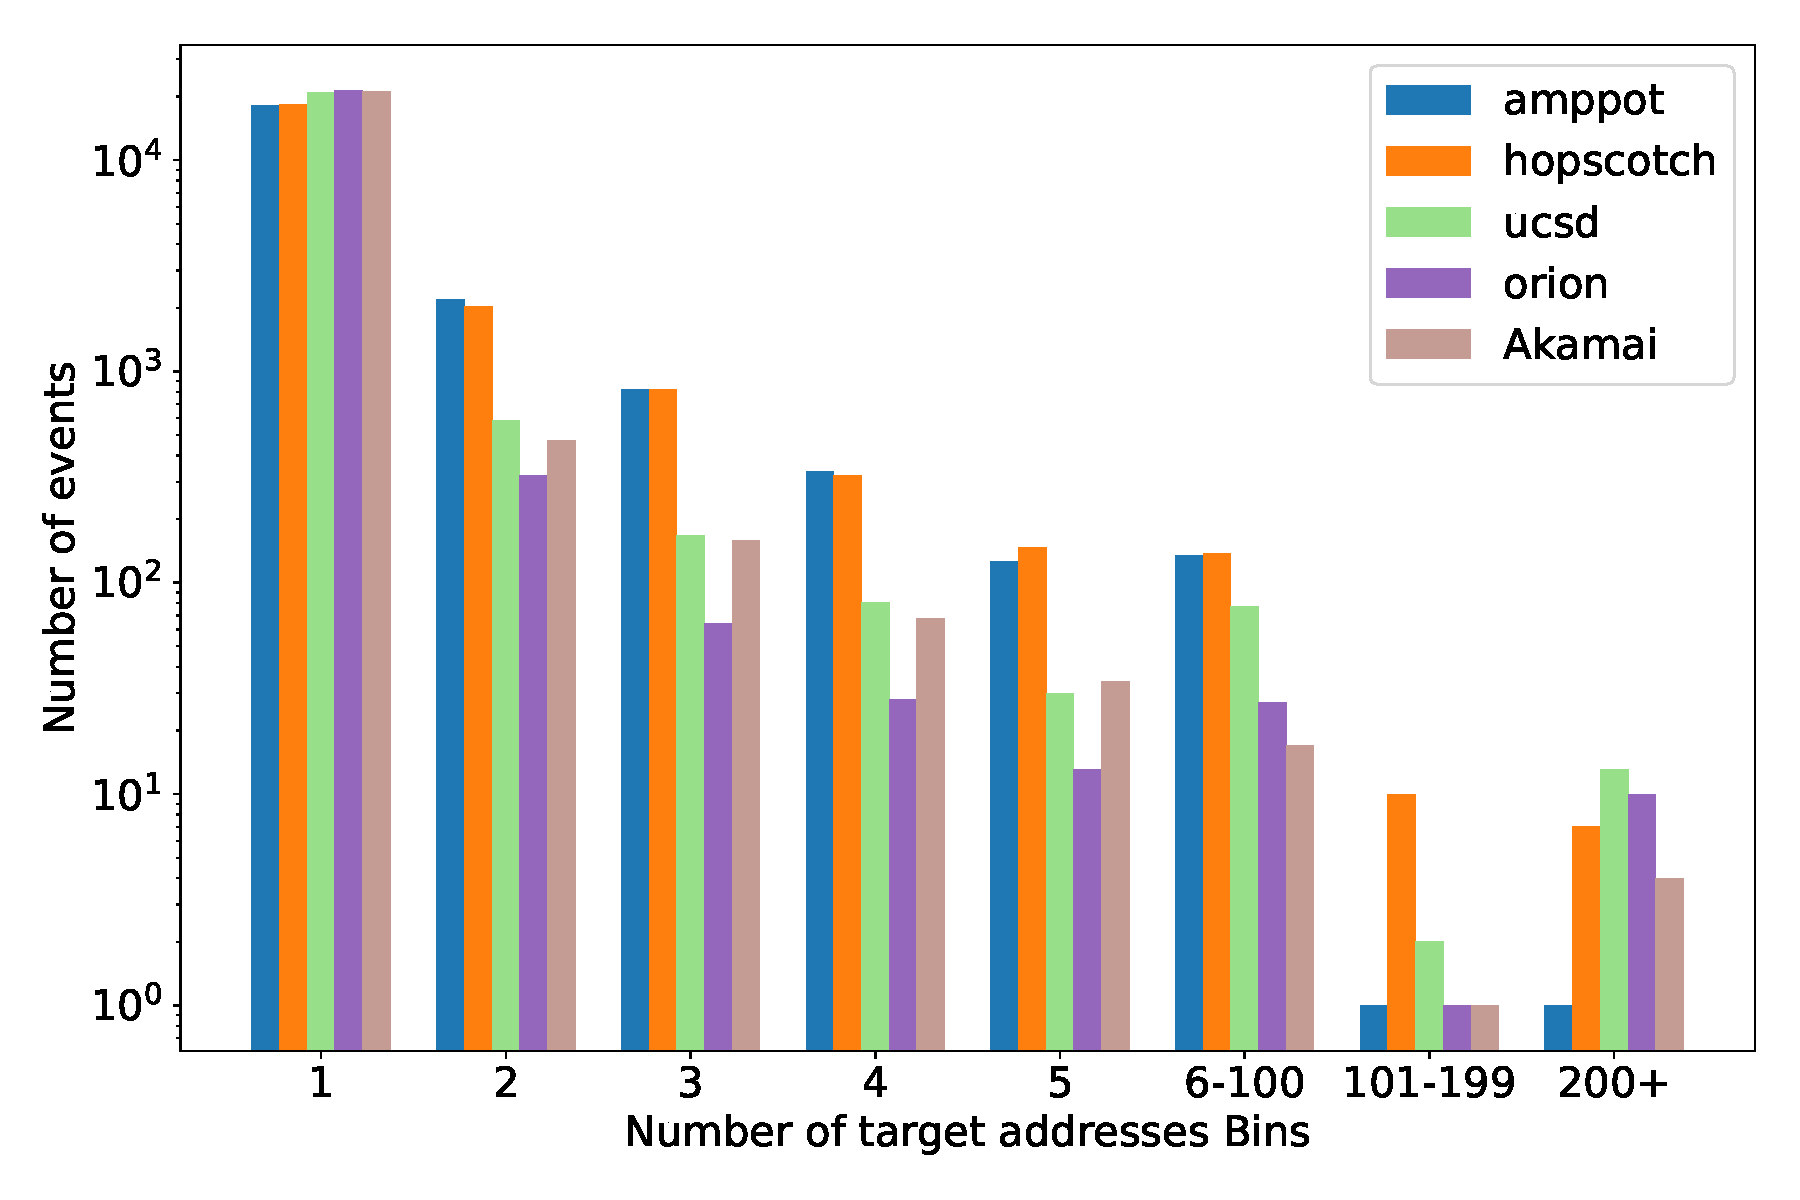
\includegraphics[scale=0.48]{graphs/bins.pdf}
    \caption{Customer IP Space and event Analysis.}
    \label{fig:akamai_spikes}
\end{figure*}
\bibliographystyle{plain}
\bibliography{akamai_ref}
\end{document}
